\section{Semantic Role Labeling}
\label{sec:srl}
Semantic Role Labeling (SRL) task aims to perform semantic analysis of texts that analyzes the propositions expressed by all target verbs of the sentence. 
For each target verb (also known as predicate), all constituents (or arguments) related to that verb are assigned semantic role labels. In common, the task is to extract predicate-argument structure for input sentences to answer the question “who did what to whom, when, where, how and why ?”.
Common solutions for the SRL can be treated as a classification problem performed on each part of the input sentence. 
The methods  aim to classify each part into correct semantic roles with respect to the predicates. \\
Many deep neural networks were proposed to solve the problem with or without detected predicates \cite{zhou2015end, marcheggiani2017simple, he2017deep, tan2018deep, he2018jointly, strubell2018linguistically}. 
The main approach is to apply the sequential models to learn the representations for each input part, then perform classification into a pre-defined set of roles.\\ 
As mentioned in section \ref{sec:BERT}, BERT is a powerful pretraining for such language modeling tasks. Shi, Peng, and Jimmy Lin.\cite{shi2019simple} proposed a BERT-based model to solve the SRL problem and achieve state-of-the-art results on different benchmarks. The method is then applied in various video-text related problems to implement such fine-grained models (discussed in section). 
\begin{figure}[t!]
    \centering
    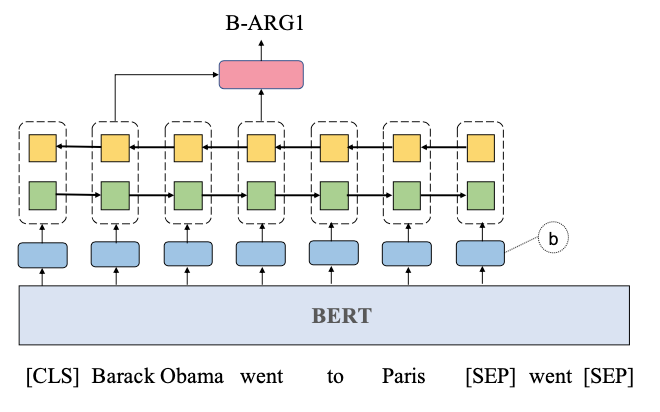
\includegraphics[width=0.7\textwidth]{resources/images/SRL_overview.png}
    \caption{An example of the BERT-based SRL method \cite{shi2019simple} making prediction for the token "Barack".}
    \label{fig:srl_overview}
\end{figure}
The architecture is constructed from BERT encoding followed by a BiLSTM layer, and a one-hidden-layer MLP to produce prediction for each tokens. In more details, the process is as follows (illustrated in figure \ref{fig:srl_overview}):
\begin{itemize}
    \item Given a pair of sentence-predicate $(X, p)$ as input, the input sequence is encoded as [[CLS] sentence [SEP] predicate [SEP]]. This method allows the predicate representation to interact with the whole input context via the self-attention mechanism.
    \item The encoded sequence is then fed into BERT encoder to obtain the sentence representations from [[CLS] sentence [SEP]] tokens. The predicate indicator embedding $\mathbf{b}$ is also associated to locate the predicate positions in the sentence.
    \item The sentence representations are then fed through a BiLSTM layer to get the final representation of each token. 
    \item Finally, to get semantic role prediction for each token, the final hidden state of predicate $\mathbf{h_p}$ is concatenated to that token hidden state $\mathbf{h_i}$ and fed into a feed-forward classifier layer over the pre-defined role set.
\end{itemize}

\textbf{SRL in vision} 
\begin{figure}[!htb]
    \centering
    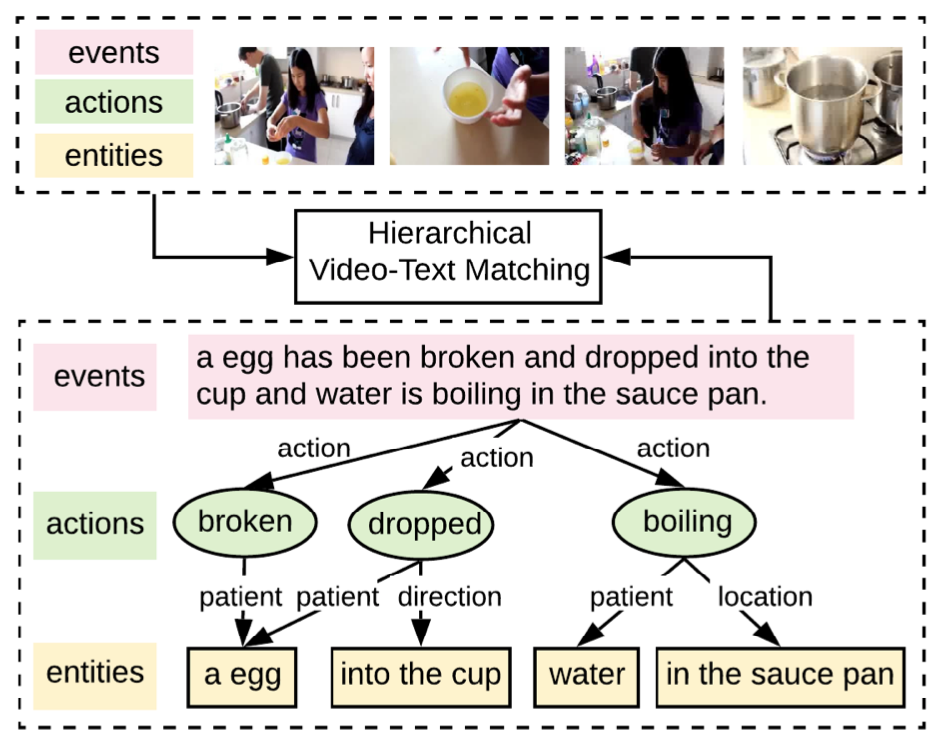
\includegraphics[width=0.7\textwidth]{resources/images/HGR_idea.png}
    \caption{The overview of HGR\cite{chen2020fine} matching process.}
    \label{fig:hgr_overview}
\end{figure}

The SRL task attracts much attention from researchers and has been widely applied in video analytics, where it provides fine-grained cues for matching textual description to correct visual context, such as human object interaction \cite{gupta2015visual}, video question answering \cite{sadhu2021video}, or video grounding \cite{sadhu2020video}, etc. The most related to ours is the utilization of SRL in video-text retrieval. Chen, Shizhe, et al. \cite{chen2020fine} proposed a Hierarchical Graph Reasoning (HGR) model to performs fine-grained retrieval task in many levels (shown in figure \ref{fig:hgr_overview}).
For each input sentence, Shizhe, et al. \cite{chen2020fine} first applies the SRL toolkit \cite{shi2019simple} to obtain predicates and their related semantic role then construct a three-level role graph, including events, actions and entities levels. 
The event node contains the whole input sentence to represent the global context, connected by action nodes that contain the extracted predicates context. The other noun phrases are entity nodes connected to different action nodes. The directed edges between action nodes and entity nodes indicate their semantic role relation.\\
In our work, the input query describes different attributes of the target objects, we apply SRL toolkit\cite{shi2019simple} to extract these signals to perform refinement and re-ranking to enhance the retrieval results.


